\documentclass{standalone}
\usepackage{amsmath,amssymb}
\usepackage{newtxtext,newtxmath}
\usepackage{xcolor}
\usepackage{tikz}
\usetikzlibrary{arrows.meta,positioning,calc,decorations.pathreplacing}

\definecolor{ink}{HTML}{1B1F23}
\definecolor{slate}{HTML}{555E68}
\definecolor{muted}{HTML}{8E96A0}
\definecolor{light}{HTML}{C6CCD2}
\definecolor{faint}{HTML}{E6E9ED}
\definecolor{quantum}{HTML}{2C5E8A}
\definecolor{quantumlight}{HTML}{6C9AC3}
\definecolor{quantumpale}{HTML}{DCE7F2}
\definecolor{ochre}{HTML}{B86B19}
\definecolor{ochrelight}{HTML}{E2B98B}
\definecolor{ochrepale}{HTML}{F6E9D8}

\newcommand{\pfmain}[1]{{\fontsize{7.6}{8.8}\selectfont\color{ink}#1}}
\newcommand{\pfsub}[1]{{\fontsize{7.0}{8.2}\selectfont\color{ink}#1}}
\newcommand{\pfslate}[1]{{\fontsize{7.0}{8.2}\selectfont\color{slate}#1}}
\newcommand{\pfquantum}[1]{{\fontsize{7.0}{8.2}\selectfont\color{quantum}#1}}
\newcommand{\pfochre}[1]{{\fontsize{7.0}{8.2}\selectfont\color{ochre}#1}}

\newcommand{\haty}{%
  \tikz[baseline=(Y.base)]{%
    \node[inner sep=0pt, outer sep=0pt] (Y) {$y$};
    \draw[line width=0.45pt, line cap=round, line join=round]
      ([xshift=0.3pt,yshift=1.25pt]Y.north west) -- ([yshift=2.45pt]Y.north) -- ([xshift=-0.3pt,yshift=1.25pt]Y.north east);
  }%
}

\tikzset{
  pfarrow/.style={-{Stealth[length=3.3pt, width=2.4pt]}, line width=0.65pt, draw=ink},
  pfmutedarrow/.style={-{Stealth[length=3.2pt, width=2.3pt]}, line width=0.60pt, draw=slate},
  pfqgate/.style={
    rectangle, draw=ink, fill=white, line width=0.65pt,
    minimum height=0.225in, inner sep=2.2pt,
    font=\fontsize{7.0}{8.0}\selectfont, text=ink
  }
}

\begin{document}
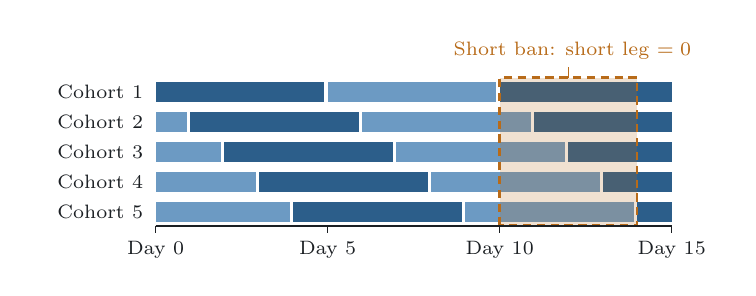
\begin{tikzpicture}[x=1in, y=1in]
  \useasboundingbox (0,0) rectangle (3.5030in, 1.20in);
  \fill[white] (0,0) rectangle (3.5030, 1.20);

  \pgfmathsetmacro{\xzero}{0.64}
  \pgfmathsetmacro{\dx}{0.172}
  \pgfmathsetmacro{\gap}{0.016}

  % Five staggered 1/5-tranche weekly cohorts with CBR short-selling ban mask
  \node[anchor=east, inner sep=0pt] at (0.58, 0.88) {\pfsub{Cohort 1}};
  \fill[quantum]      ({\xzero + 0*\dx}, 0.83) rectangle ({\xzero + 5*\dx - \gap}, 0.93);
  \fill[quantumlight] ({\xzero + 5*\dx}, 0.83) rectangle ({\xzero + 10*\dx - \gap}, 0.93);
  \fill[quantum]      ({\xzero + 10*\dx}, 0.83) rectangle ({\xzero + 15*\dx}, 0.93);

  \node[anchor=east, inner sep=0pt] at (0.58, 0.73) {\pfsub{Cohort 2}};
  \fill[quantumlight] ({\xzero + 0*\dx}, 0.68) rectangle ({\xzero + 1*\dx - \gap}, 0.78);
  \fill[quantum]      ({\xzero + 1*\dx}, 0.68) rectangle ({\xzero + 6*\dx - \gap}, 0.78);
  \fill[quantumlight] ({\xzero + 6*\dx}, 0.68) rectangle ({\xzero + 11*\dx - \gap}, 0.78);
  \fill[quantum]      ({\xzero + 11*\dx}, 0.68) rectangle ({\xzero + 15*\dx}, 0.78);

  \node[anchor=east, inner sep=0pt] at (0.58, 0.58) {\pfsub{Cohort 3}};
  \fill[quantumlight] ({\xzero + 0*\dx}, 0.53) rectangle ({\xzero + 2*\dx - \gap}, 0.63);
  \fill[quantum]      ({\xzero + 2*\dx}, 0.53) rectangle ({\xzero + 7*\dx - \gap}, 0.63);
  \fill[quantumlight] ({\xzero + 7*\dx}, 0.53) rectangle ({\xzero + 12*\dx - \gap}, 0.63);
  \fill[quantum]      ({\xzero + 12*\dx}, 0.53) rectangle ({\xzero + 15*\dx}, 0.63);

  \node[anchor=east, inner sep=0pt] at (0.58, 0.43) {\pfsub{Cohort 4}};
  \fill[quantumlight] ({\xzero + 0*\dx}, 0.38) rectangle ({\xzero + 3*\dx - \gap}, 0.48);
  \fill[quantum]      ({\xzero + 3*\dx}, 0.38) rectangle ({\xzero + 8*\dx - \gap}, 0.48);
  \fill[quantumlight] ({\xzero + 8*\dx}, 0.38) rectangle ({\xzero + 13*\dx - \gap}, 0.48);
  \fill[quantum]      ({\xzero + 13*\dx}, 0.38) rectangle ({\xzero + 15*\dx}, 0.48);

  \node[anchor=east, inner sep=0pt] at (0.58, 0.28) {\pfsub{Cohort 5}};
  \fill[quantumlight] ({\xzero + 0*\dx}, 0.23) rectangle ({\xzero + 4*\dx - \gap}, 0.33);
  \fill[quantum]      ({\xzero + 4*\dx}, 0.23) rectangle ({\xzero + 9*\dx - \gap}, 0.33);
  \fill[quantumlight] ({\xzero + 9*\dx}, 0.23) rectangle ({\xzero + 14*\dx - \gap}, 0.33);
  \fill[quantum]      ({\xzero + 14*\dx}, 0.23) rectangle ({\xzero + 15*\dx}, 0.33);

  \fill[ochre, fill opacity=0.20] ({\xzero + 10*\dx}, 0.21) rectangle ({\xzero + 14*\dx}, 0.95);
  \draw[ochre, line width=0.85pt, densely dashed] ({\xzero + 10*\dx}, 0.21) rectangle ({\xzero + 14*\dx}, 0.95);
  \node[anchor=east, inner sep=0pt] at (3.32, 1.085) {\pfochre{Short ban: short leg $= 0$}};
  \draw[ochre, line width=0.60pt] ({\xzero + 12*\dx}, 0.95) -- ({\xzero + 12*\dx}, 1.005);

  \draw[ink, line width=0.60pt] (\xzero, 0.21) -- ({\xzero + 15*\dx}, 0.21);
  \foreach \s/\slbl in {0/{Day 0}, 5/{Day 5}, 10/{Day 10}, 15/{Day 15}} {
    \draw[ink, line width=0.55pt] ({\xzero + \s*\dx}, 0.21) -- ({\xzero + \s*\dx}, 0.175);
    \node[anchor=north, inner sep=0pt] at ({\xzero + \s*\dx}, 0.135) {\pfsub{\slbl}};
  }
\end{tikzpicture}
\end{document}
